\documentclass[twoside]{book}

% Packages required by doxygen
\usepackage{fixltx2e}
\usepackage{calc}
\usepackage{doxygen}
\usepackage[export]{adjustbox} % also loads graphicx
\usepackage{graphicx}
\usepackage[utf8]{inputenc}
\usepackage{makeidx}
\usepackage{multicol}
\usepackage{multirow}
\PassOptionsToPackage{warn}{textcomp}
\usepackage{textcomp}
\usepackage[nointegrals]{wasysym}
\usepackage[table]{xcolor}

% Font selection
\usepackage[T1]{fontenc}
\usepackage[scaled=.90]{helvet}
\usepackage{courier}
\usepackage{amssymb}
\usepackage{sectsty}
\renewcommand{\familydefault}{\sfdefault}
\allsectionsfont{%
  \fontseries{bc}\selectfont%
  \color{darkgray}%
}
\renewcommand{\DoxyLabelFont}{%
  \fontseries{bc}\selectfont%
  \color{darkgray}%
}
\newcommand{\+}{\discretionary{\mbox{\scriptsize$\hookleftarrow$}}{}{}}

% Page & text layout
\usepackage{geometry}
\geometry{%
  a4paper,%
  top=2.5cm,%
  bottom=2.5cm,%
  left=2.5cm,%
  right=2.5cm%
}
\tolerance=750
\hfuzz=15pt
\hbadness=750
\setlength{\emergencystretch}{15pt}
\setlength{\parindent}{0cm}
\setlength{\parskip}{3ex plus 2ex minus 2ex}
\makeatletter
\renewcommand{\paragraph}{%
  \@startsection{paragraph}{4}{0ex}{-1.0ex}{1.0ex}{%
    \normalfont\normalsize\bfseries\SS@parafont%
  }%
}
\renewcommand{\subparagraph}{%
  \@startsection{subparagraph}{5}{0ex}{-1.0ex}{1.0ex}{%
    \normalfont\normalsize\bfseries\SS@subparafont%
  }%
}
\makeatother

% Headers & footers
\usepackage{fancyhdr}
\pagestyle{fancyplain}
\fancyhead[LE]{\fancyplain{}{\bfseries\thepage}}
\fancyhead[CE]{\fancyplain{}{}}
\fancyhead[RE]{\fancyplain{}{\bfseries\leftmark}}
\fancyhead[LO]{\fancyplain{}{\bfseries\rightmark}}
\fancyhead[CO]{\fancyplain{}{}}
\fancyhead[RO]{\fancyplain{}{\bfseries\thepage}}
\fancyfoot[LE]{\fancyplain{}{}}
\fancyfoot[CE]{\fancyplain{}{}}
\fancyfoot[RE]{\fancyplain{}{\bfseries\scriptsize Generated by Doxygen }}
\fancyfoot[LO]{\fancyplain{}{\bfseries\scriptsize Generated by Doxygen }}
\fancyfoot[CO]{\fancyplain{}{}}
\fancyfoot[RO]{\fancyplain{}{}}
\renewcommand{\footrulewidth}{0.4pt}
\renewcommand{\chaptermark}[1]{%
  \markboth{#1}{}%
}
\renewcommand{\sectionmark}[1]{%
  \markright{\thesection\ #1}%
}

% Indices & bibliography
\usepackage{natbib}
\usepackage[titles]{tocloft}
\setcounter{tocdepth}{3}
\setcounter{secnumdepth}{5}
\makeindex

% Hyperlinks (required, but should be loaded last)
\usepackage{ifpdf}
\ifpdf
  \usepackage[pdftex,pagebackref=true]{hyperref}
\else
  \usepackage[ps2pdf,pagebackref=true]{hyperref}
\fi
\hypersetup{%
  colorlinks=true,%
  linkcolor=blue,%
  citecolor=blue,%
  unicode%
}

% Custom commands
\newcommand{\clearemptydoublepage}{%
  \newpage{\pagestyle{empty}\cleardoublepage}%
}

\usepackage{caption}
\captionsetup{labelsep=space,justification=centering,font={bf},singlelinecheck=off,skip=4pt,position=top}

%===== C O N T E N T S =====

\begin{document}

% Titlepage & ToC
\hypersetup{pageanchor=false,
             bookmarksnumbered=true,
             pdfencoding=unicode
            }
\pagenumbering{alph}
\begin{titlepage}
\vspace*{7cm}
\begin{center}%
{\Large My Project }\\
\vspace*{1cm}
{\large Generated by Doxygen 1.8.13}\\
\end{center}
\end{titlepage}
\clearemptydoublepage
\pagenumbering{roman}
\tableofcontents
\clearemptydoublepage
\pagenumbering{arabic}
\hypersetup{pageanchor=true}

%--- Begin generated contents ---
\chapter{Firmware alpha}
\label{md_README}
\Hypertarget{md_README}
This repository is an open-\/source autopilot developed with Platform\+IO and Visual Studio Code. It is compatible with \href{https://os.mbed.com/mbed-os/}{\tt A\+RM\textregistered{} Mbed\texttrademark{} OS} and makes use of its A\+P\+Is. The autopilot is tested on a \href{https://os.mbed.com/platforms/FRDM-K64F/}{\tt N\+XP F\+R\+D\+M-\/\+K64F} board. \subsection*{Processor-\/\+In-\/the-\/\+Loop (P\+IL)}

{\itshape Processor-\/\+In-\/the-\/\+Loop} validation allows the developer to test the software directly on the target board. The board is connected with an external PC on which is running the physical model of the robot as well as a model of its actuators and sensors. This firmware supports communication using the {\bfseries U\+DP} protocol to talk with the external PC. The connection properties (e.\+g. IP, Port...) can be modified in the file {\itshape U\+D\+P\+Comm.\+cpp}\+: 
\begin{DoxyCode}
\{c++\}
static const char*          mbedIP       = "192.168.1.55";      // This board IP seen from the network
static const char*          mbedMask     = "255.255.255.0";     // Mask
static const char*          mbedGateway  = "192.168.1.254";     // Gateway

static const char*          recvIP = "192.168.1.203";           // External PC IP */ "192.168.1.249";
static const char*          localIP = "0.0.0.0";                // Local IP on which the server of the
       board listens
\end{DoxyCode}
 The messaging protocol used is \href{https://mavlink.io/en/}{\tt Mavlink v2.\+0} since it is lightweight, open-\/source and widespread. \subsubsection*{P\+IL with Matlab/\+Simulink\textregistered{}}

It is possible to employ Simulink to create the robot model

\subsection*{Code generation with Matlab/\+Simulink\textregistered{}}

For {\itshape Rapid Prototyping} purposes, code generation is a valid tool. The Firmware is compatible with C/\+C++ code automatically generated from Matlab/\+Simulink\textregistered{}. Here general rules and the settings used in the {\bfseries Model Configuration Parameter} pane are shown so that scripts generated by the embedded coder in Simulink are compatible with the Firmware. \paragraph*{General rules}

The following general rules have to be taken into account when creating the Simulink model\+:
\begin{DoxyItemize}
\item To match the variable names in the Firmware, the Simulink model has to be named \char`\"{}$\ast$feedback\+\_\+control.\+slx$\ast$\char`\"{}, so that input and output variables are structs named respectively {\itshape feedback\+\_\+control\+\_\+U} and {\itshape feedback\+\_\+control\+\_\+Y};
\item The {\bfseries In1} and {\bfseries Out1} ports in Simulink has to be carefully named since the arguments of the C++ controller step function are structs whose members take the name from those ports. \paragraph*{Interface}
\end{DoxyItemize}

\subsubsection*{Firmware with generated code}

The generated code can be easily added to the Firmware by doing a copy and paste of the header files into the {\itshape include} folder and the source files into the {\itshape src} folder. Then, few modifications have to be done to make the Firmware compatible with some generated code\+:
\begin{DoxyItemize}
\item Look throughout the scripts depending on the header {\itshape \hyperlink{global__vars_8hpp}{global\+\_\+vars.\+hpp}} and add the {\itshape feedback\+\_\+control\+\_\+U} and {\itshape feedback\+\_\+control\+\_\+Y} structs 
\end{DoxyItemize}
\chapter{File Index}
\section{File List}
Here is a list of all documented files with brief descriptions\+:\begin{DoxyCompactList}
\item\contentsline{section}{include/\hyperlink{global__vars_8hpp}{global\+\_\+vars.\+hpp} \\*Header gathering the global variables used in the Firmware }{\pageref{global__vars_8hpp}}{}
\item\contentsline{section}{src/\hyperlink{main_8cpp}{main.\+cpp} \\*Entry point for mbed OS }{\pageref{main_8cpp}}{}
\item\contentsline{section}{src/\hyperlink{sensInit_8cpp}{sens\+Init.\+cpp} \\*Thread initializing sensors read at the given frequency }{\pageref{sensInit_8cpp}}{}
\item\contentsline{section}{src/\hyperlink{UDPComm_8cpp}{U\+D\+P\+Comm.\+cpp} \\*Enables U\+DP communication between the target board and an external PC to perform Processor-\/\+In-\/the-\/\+Loop }{\pageref{UDPComm_8cpp}}{}
\end{DoxyCompactList}

\chapter{File Documentation}
\hypertarget{global__vars_8hpp}{}\section{include/global\+\_\+vars.hpp File Reference}
\label{global__vars_8hpp}\index{include/global\+\_\+vars.\+hpp@{include/global\+\_\+vars.\+hpp}}


Header gathering the global variables used in the Firmware.  


{\ttfamily \#include $<$mbed.\+h$>$}\newline
{\ttfamily \#include \char`\"{}common/mavlink.\+h\char`\"{}}\newline
{\ttfamily \#include \char`\"{}feedback\+\_\+control.\+h\char`\"{}}\newline
{\ttfamily \#include \char`\"{}Servo.\+h\char`\"{}}\newline
This graph shows which files directly or indirectly include this file\+:
\nopagebreak
\begin{figure}[H]
\begin{center}
\leavevmode
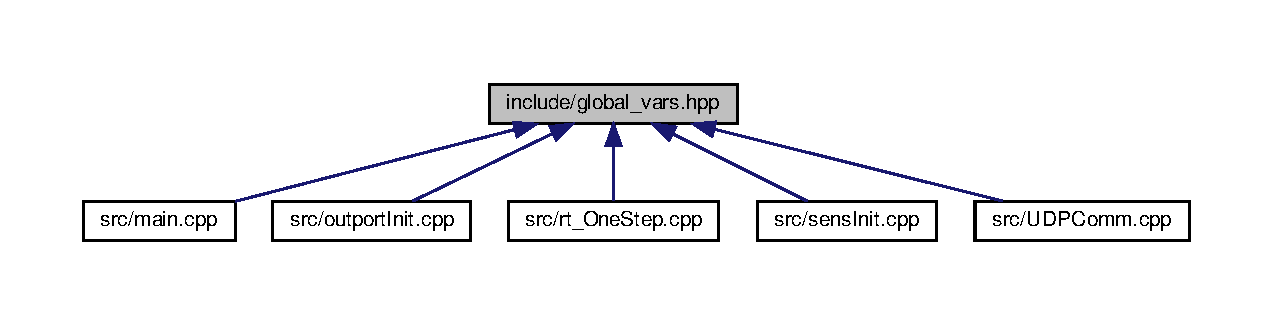
\includegraphics[width=199pt]{global__vars_8hpp__dep__incl}
\end{center}
\end{figure}
\subsection*{Variables}
\begin{DoxyCompactItemize}
\item 
Ext\+U\+\_\+feedback\+\_\+control\+\_\+T \hyperlink{global__vars_8hpp_a1bfda025b86a8da3a44e6b0923a256f2}{feedback\+\_\+control\+\_\+U}
\item 
Ext\+Y\+\_\+feedback\+\_\+control\+\_\+T \hyperlink{global__vars_8hpp_ae01be5449c13f73da04804c6c995d2ea}{feedback\+\_\+control\+\_\+Y}
\item 
\mbox{\Hypertarget{global__vars_8hpp_aaf3aa91f66e97e290265d2078ba3b1ad}\label{global__vars_8hpp_aaf3aa91f66e97e290265d2078ba3b1ad}} 
Semaphore {\bfseries sem\+Decode}
\item 
\mbox{\Hypertarget{global__vars_8hpp_a414bcf18f502e41c624ce447862af727}\label{global__vars_8hpp_a414bcf18f502e41c624ce447862af727}} 
Semaphore {\bfseries sem\+Encode}
\item 
\mbox{\Hypertarget{global__vars_8hpp_ac5d2bea44c6318454db0e2639a4efe95}\label{global__vars_8hpp_ac5d2bea44c6318454db0e2639a4efe95}} 
Servo {\bfseries servo1}
\item 
\mbox{\Hypertarget{global__vars_8hpp_ac158b76bc8e2f8f232c4b8a73d1a2cb2}\label{global__vars_8hpp_ac158b76bc8e2f8f232c4b8a73d1a2cb2}} 
Event\+Queue {\bfseries queue}
\end{DoxyCompactItemize}


\subsection{Detailed Description}
Header gathering the global variables used in the Firmware. 

Global variables are chosen upon u\+O\+RB because yes. 

\subsection{Variable Documentation}
\mbox{\Hypertarget{global__vars_8hpp_a1bfda025b86a8da3a44e6b0923a256f2}\label{global__vars_8hpp_a1bfda025b86a8da3a44e6b0923a256f2}} 
\index{global\+\_\+vars.\+hpp@{global\+\_\+vars.\+hpp}!feedback\+\_\+control\+\_\+U@{feedback\+\_\+control\+\_\+U}}
\index{feedback\+\_\+control\+\_\+U@{feedback\+\_\+control\+\_\+U}!global\+\_\+vars.\+hpp@{global\+\_\+vars.\+hpp}}
\subsubsection{\texorpdfstring{feedback\+\_\+control\+\_\+U}{feedback\_control\_U}}
{\footnotesize\ttfamily Ext\+U\+\_\+feedback\+\_\+control\+\_\+T feedback\+\_\+control\+\_\+U}

The I/O variables of the controller are used as extern since their name is the same if a Simulink project is used. This allows to keep the Firmware unchanged.\+External inputs \mbox{\Hypertarget{global__vars_8hpp_ae01be5449c13f73da04804c6c995d2ea}\label{global__vars_8hpp_ae01be5449c13f73da04804c6c995d2ea}} 
\index{global\+\_\+vars.\+hpp@{global\+\_\+vars.\+hpp}!feedback\+\_\+control\+\_\+Y@{feedback\+\_\+control\+\_\+Y}}
\index{feedback\+\_\+control\+\_\+Y@{feedback\+\_\+control\+\_\+Y}!global\+\_\+vars.\+hpp@{global\+\_\+vars.\+hpp}}
\subsubsection{\texorpdfstring{feedback\+\_\+control\+\_\+Y}{feedback\_control\_Y}}
{\footnotesize\ttfamily Ext\+Y\+\_\+feedback\+\_\+control\+\_\+T feedback\+\_\+control\+\_\+Y}

External outputs 
\hypertarget{cli2_8cpp}{}\section{src/cli2.cpp File Reference}
\label{cli2_8cpp}\index{src/cli2.\+cpp@{src/cli2.\+cpp}}


Command line interface for hardware resource inspection.  


{\ttfamily \#include \char`\"{}cli2.\+hpp\char`\"{}}\newline
{\ttfamily \#include \char`\"{}sysinfo.\+hpp\char`\"{}}\newline
{\ttfamily \#include \char`\"{}top.\+hpp\char`\"{}}\newline
{\ttfamily \#include \char`\"{}threadinfo.\+hpp\char`\"{}}\newline
{\ttfamily \#include \char`\"{}cli\+\_\+appereance.\+hpp\char`\"{}}\newline
Include dependency graph for cli2.\+cpp\+:\nopagebreak
\begin{figure}[H]
\begin{center}
\leavevmode
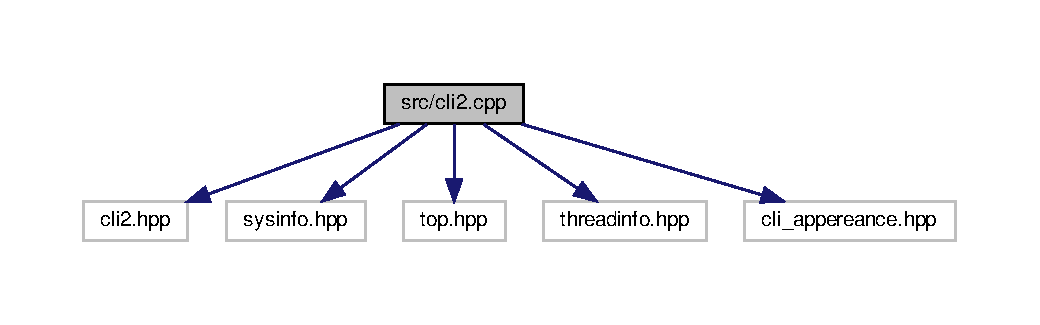
\includegraphics[width=350pt]{cli2_8cpp__incl}
\end{center}
\end{figure}


\subsection{Detailed Description}
Command line interface for hardware resource inspection. 

The command line interface (cli) allows the developer to check the C\+PU and memory usage, the number of active threads and display the main variables. The available commands are\+:
\begin{DoxyItemize}
\item top Display C\+PU usage;
\item info Display hardware information;
\item thread Show active threads state, priority and their resources;
\item clear Clear screen;
\item help Show available commands. 
\end{DoxyItemize}
\hypertarget{main_8cpp}{}\section{src/main.cpp File Reference}
\label{main_8cpp}\index{src/main.\+cpp@{src/main.\+cpp}}


Entry point for mbed OS.  


{\ttfamily \#include $<$mbed.\+h$>$}\newline
{\ttfamily \#include $<$Serial.\+h$>$}\newline
{\ttfamily \#include $<$Ethernet\+Interface.\+h$>$}\newline
{\ttfamily \#include \char`\"{}global\+\_\+vars.\+hpp\char`\"{}}\newline
{\ttfamily \#include \char`\"{}common/mavlink.\+h\char`\"{}}\newline
{\ttfamily \#include \char`\"{}cntr\+Init.\+hpp\char`\"{}}\newline
{\ttfamily \#include \char`\"{}sens\+Init.\+hpp\char`\"{}}\newline
{\ttfamily \#include \char`\"{}outport\+Init.\+hpp\char`\"{}}\newline
{\ttfamily \#include \char`\"{}cli2.\+hpp\char`\"{}}\newline
Include dependency graph for main.\+cpp\+:\nopagebreak
\begin{figure}[H]
\begin{center}
\leavevmode
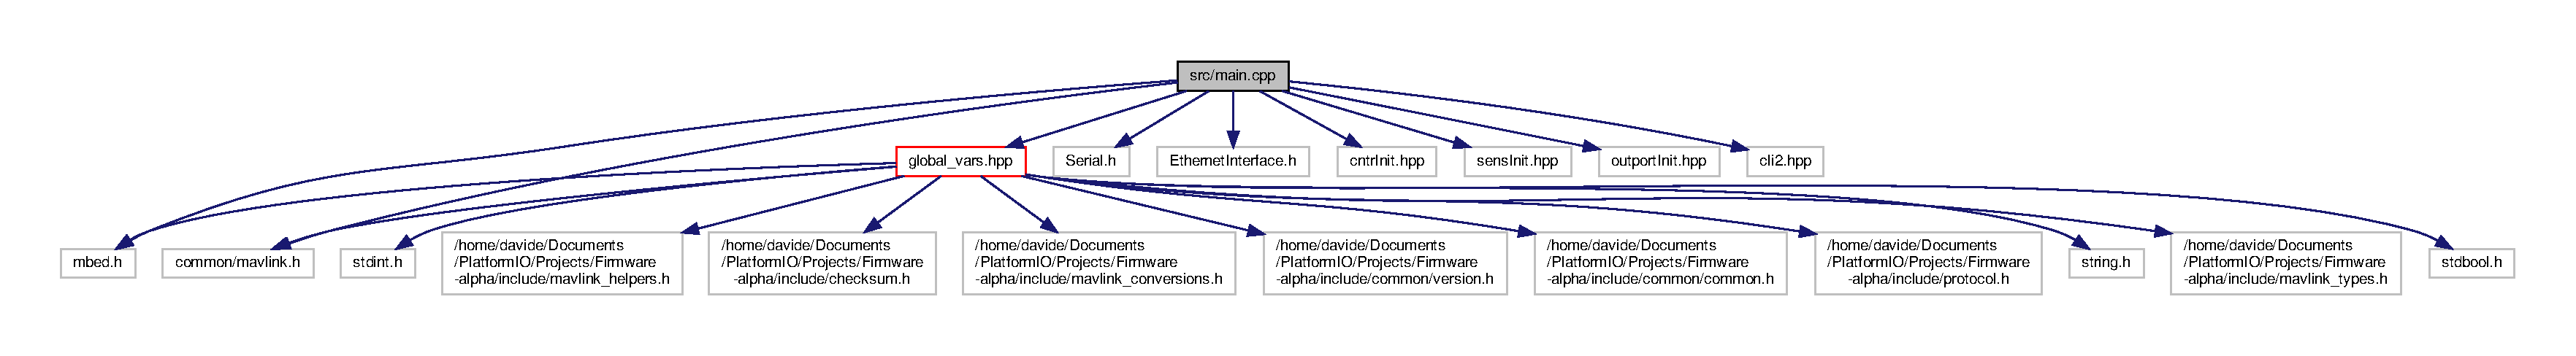
\includegraphics[width=350pt]{main_8cpp__incl}
\end{center}
\end{figure}
\subsection*{Variables}
\begin{DoxyCompactItemize}
\item 
Ext\+U\+\_\+feedback\+\_\+control\+\_\+T \hyperlink{main_8cpp_a1bfda025b86a8da3a44e6b0923a256f2}{feedback\+\_\+control\+\_\+U}
\item 
Ext\+Y\+\_\+feedback\+\_\+control\+\_\+T \hyperlink{main_8cpp_ae01be5449c13f73da04804c6c995d2ea}{feedback\+\_\+control\+\_\+Y}
\end{DoxyCompactItemize}


\subsection{Detailed Description}
Entry point for mbed OS. 

This script creates and spawns threads and declare global variables defined in the header \hyperlink{global__vars_8hpp}{global\+\_\+vars.\+hpp}. 

\subsection{Variable Documentation}
\mbox{\Hypertarget{main_8cpp_a1bfda025b86a8da3a44e6b0923a256f2}\label{main_8cpp_a1bfda025b86a8da3a44e6b0923a256f2}} 
\index{main.\+cpp@{main.\+cpp}!feedback\+\_\+control\+\_\+U@{feedback\+\_\+control\+\_\+U}}
\index{feedback\+\_\+control\+\_\+U@{feedback\+\_\+control\+\_\+U}!main.\+cpp@{main.\+cpp}}
\subsubsection{\texorpdfstring{feedback\+\_\+control\+\_\+U}{feedback\_control\_U}}
{\footnotesize\ttfamily Ext\+U\+\_\+feedback\+\_\+control\+\_\+T feedback\+\_\+control\+\_\+U}

The I/O variables of the controller are used as extern since their name is the same if a Simulink project is used. This allows to keep the Firmware unchanged.\+External inputs \mbox{\Hypertarget{main_8cpp_ae01be5449c13f73da04804c6c995d2ea}\label{main_8cpp_ae01be5449c13f73da04804c6c995d2ea}} 
\index{main.\+cpp@{main.\+cpp}!feedback\+\_\+control\+\_\+Y@{feedback\+\_\+control\+\_\+Y}}
\index{feedback\+\_\+control\+\_\+Y@{feedback\+\_\+control\+\_\+Y}!main.\+cpp@{main.\+cpp}}
\subsubsection{\texorpdfstring{feedback\+\_\+control\+\_\+Y}{feedback\_control\_Y}}
{\footnotesize\ttfamily Ext\+Y\+\_\+feedback\+\_\+control\+\_\+T feedback\+\_\+control\+\_\+Y}

External outputs 
\hypertarget{outportInit_8cpp}{}\section{src/outport\+Init.cpp File Reference}
\label{outportInit_8cpp}\index{src/outport\+Init.\+cpp@{src/outport\+Init.\+cpp}}


This thread creates the periodic task sending the pulse-\/width modulated signals to the enabled pins.  


{\ttfamily \#include $<$mbed.\+h$>$}\newline
{\ttfamily \#include \char`\"{}Servo.\+h\char`\"{}}\newline
{\ttfamily \#include \char`\"{}global\+\_\+vars.\+hpp\char`\"{}}\newline
{\ttfamily \#include \char`\"{}outport\+Init.\+hpp\char`\"{}}\newline
Include dependency graph for outport\+Init.\+cpp\+:\nopagebreak
\begin{figure}[H]
\begin{center}
\leavevmode
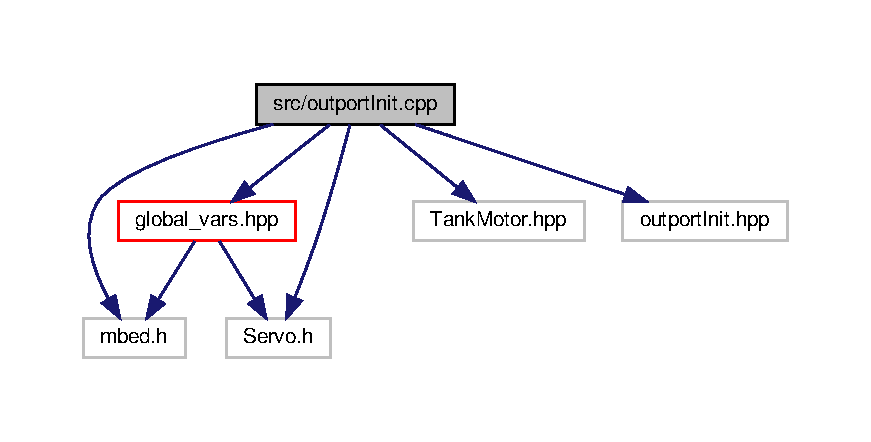
\includegraphics[width=318pt]{outportInit_8cpp__incl}
\end{center}
\end{figure}
\subsection*{Functions}
\begin{DoxyCompactItemize}
\item 
void \hyperlink{outportInit_8cpp_a2932cb03107afa47dfd97b8547333d8f}{outport\+Init} ()
\item 
void \hyperlink{outportInit_8cpp_a44135f9954133bdb9393bc4ca364732f}{post\+Servo\+Event} (void)
\item 
void \hyperlink{outportInit_8cpp_a0b36bbd1441854181e55a0d94af7345f}{Servo1\+Write} (void)
\end{DoxyCompactItemize}


\subsection{Detailed Description}
This thread creates the periodic task sending the pulse-\/width modulated signals to the enabled pins. 

\begin{DoxyAuthor}{Author}
Davide Carminati
\end{DoxyAuthor}
The script uses events and a queue to pile periodic tasks. The queue contains both read-\/from and write-\/to pins events. 

\subsection{Function Documentation}
\mbox{\Hypertarget{outportInit_8cpp_a2932cb03107afa47dfd97b8547333d8f}\label{outportInit_8cpp_a2932cb03107afa47dfd97b8547333d8f}} 
\index{outport\+Init.\+cpp@{outport\+Init.\+cpp}!outport\+Init@{outport\+Init}}
\index{outport\+Init@{outport\+Init}!outport\+Init.\+cpp@{outport\+Init.\+cpp}}
\subsubsection{\texorpdfstring{outport\+Init()}{outportInit()}}
{\footnotesize\ttfamily void outport\+Init (\begin{DoxyParamCaption}{ }\end{DoxyParamCaption})}

Initialization of the servomotor, spawn of the event posting thread and dispatch queue. The Servo\+::calibrate() method accepts as first input a value IN S\+E\+C\+O\+N\+DS. \mbox{\Hypertarget{outportInit_8cpp_a44135f9954133bdb9393bc4ca364732f}\label{outportInit_8cpp_a44135f9954133bdb9393bc4ca364732f}} 
\index{outport\+Init.\+cpp@{outport\+Init.\+cpp}!post\+Servo\+Event@{post\+Servo\+Event}}
\index{post\+Servo\+Event@{post\+Servo\+Event}!outport\+Init.\+cpp@{outport\+Init.\+cpp}}
\subsubsection{\texorpdfstring{post\+Servo\+Event()}{postServoEvent()}}
{\footnotesize\ttfamily void post\+Servo\+Event (\begin{DoxyParamCaption}\item[{void}]{ }\end{DoxyParamCaption})}

The period and the initial delay of the P\+WM write event are set. Then it is posted in the queue. \mbox{\Hypertarget{outportInit_8cpp_a0b36bbd1441854181e55a0d94af7345f}\label{outportInit_8cpp_a0b36bbd1441854181e55a0d94af7345f}} 
\index{outport\+Init.\+cpp@{outport\+Init.\+cpp}!Servo1\+Write@{Servo1\+Write}}
\index{Servo1\+Write@{Servo1\+Write}!outport\+Init.\+cpp@{outport\+Init.\+cpp}}
\subsubsection{\texorpdfstring{Servo1\+Write()}{Servo1Write()}}
{\footnotesize\ttfamily void Servo1\+Write (\begin{DoxyParamCaption}\item[{void}]{ }\end{DoxyParamCaption})}

The event is simply a method writing the computed duty cycle to the enabled pin port. The duty cycle is directly dependent on the output of the controller thread\+: note that the extern variable feedback\+\_\+control\+\_\+Y is present. 
\hypertarget{rt__OneStep_8cpp}{}\section{src/rt\+\_\+\+One\+Step.cpp File Reference}
\label{rt__OneStep_8cpp}\index{src/rt\+\_\+\+One\+Step.\+cpp@{src/rt\+\_\+\+One\+Step.\+cpp}}


It performs a time step of the controller algorithm checking whether it respects the Real-\/\+Time deadline.  


{\ttfamily \#include $<$stddef.\+h$>$}\newline
{\ttfamily \#include $<$stdio.\+h$>$}\newline
{\ttfamily \#include \char`\"{}feedback\+\_\+control.\+h\char`\"{}}\newline
{\ttfamily \#include \char`\"{}rtwtypes.\+h\char`\"{}}\newline
{\ttfamily \#include \char`\"{}global\+\_\+vars.\+hpp\char`\"{}}\newline
{\ttfamily \#include \char`\"{}common/mavlink.\+h\char`\"{}}\newline
{\ttfamily \#include \char`\"{}rt\+\_\+\+One\+Step.\+hpp\char`\"{}}\newline
Include dependency graph for rt\+\_\+\+One\+Step.\+cpp\+:\nopagebreak
\begin{figure}[H]
\begin{center}
\leavevmode
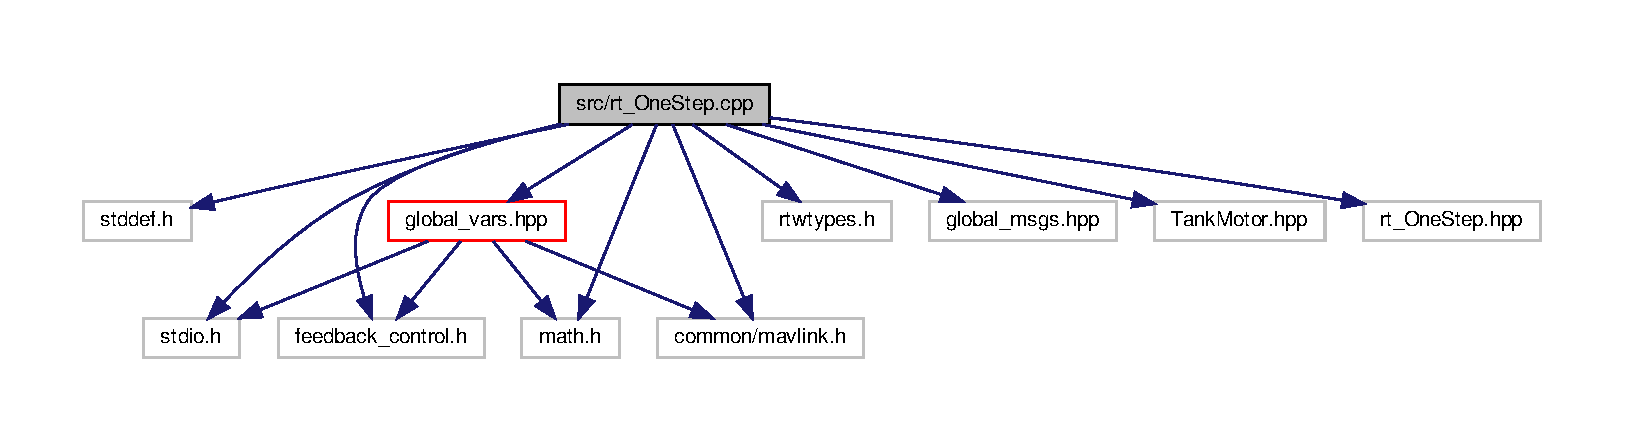
\includegraphics[width=350pt]{rt__OneStep_8cpp__incl}
\end{center}
\end{figure}


\subsection{Detailed Description}
It performs a time step of the controller algorithm checking whether it respects the Real-\/\+Time deadline. 


\hypertarget{sensInit_8cpp}{}\section{src/sens\+Init.cpp File Reference}
\label{sensInit_8cpp}\index{src/sens\+Init.\+cpp@{src/sens\+Init.\+cpp}}


Thread initializing sensors read at the given frequency.  


{\ttfamily \#include $<$mbed.\+h$>$}\newline
{\ttfamily \#include \char`\"{}F\+X\+O\+S8700\+C\+Q.\+h\char`\"{}}\newline
{\ttfamily \#include \char`\"{}global\+\_\+vars.\+hpp\char`\"{}}\newline
{\ttfamily \#include \char`\"{}sens\+Init.\+hpp\char`\"{}}\newline
{\ttfamily \#include \char`\"{}Event\+Queue.\+h\char`\"{}}\newline
{\ttfamily \#include \char`\"{}Event.\+h\char`\"{}}\newline
Include dependency graph for sens\+Init.\+cpp\+:
\nopagebreak
\begin{figure}[H]
\begin{center}
\leavevmode
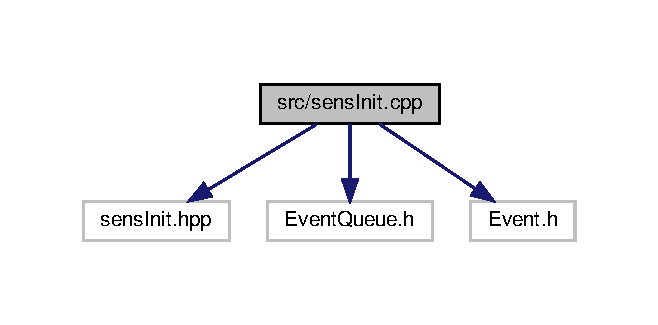
\includegraphics[width=350pt]{sensInit_8cpp__incl}
\end{center}
\end{figure}
\subsection*{Macros}
\begin{DoxyCompactItemize}
\item 
\mbox{\Hypertarget{sensInit_8cpp_afc65ba37dbbaa203d226e7fe6326adc5}\label{sensInit_8cpp_afc65ba37dbbaa203d226e7fe6326adc5}} 
\#define \hyperlink{sensInit_8cpp_afc65ba37dbbaa203d226e7fe6326adc5}{F\+X\+O\+S8700\+C\+Q\+\_\+\+F\+R\+EQ}~50
\begin{DoxyCompactList}\small\item\em Frequency at which the sensor is interrogated. \end{DoxyCompactList}\end{DoxyCompactItemize}


\subsection{Detailed Description}
Thread initializing sensors read at the given frequency. 

Creates a timer that calls an interrupt with the given frequency 
\input{UDPMavlink_8cpp}
%--- End generated contents ---

% Index
\backmatter
\newpage
\phantomsection
\clearemptydoublepage
\addcontentsline{toc}{chapter}{Index}
\printindex

\end{document}
